\section{Auswertung}
\subsection{Pockelseffekt}
Zur Auswertung des Pockelseffekt werden die Elektrooptischen Konstanten auf zwei Arten bestimmt. \par
Für die Auswertung der Methode bei der eine Sägezahnspannung an den Pockelszellen angelegt wurde werden als erstes die $15$ Datensätze geplottet und mit dem Python Packet \verb|scipy.optimize| über \verb|curve_fit| angepasst. Hierbei wurde für den anstieg der Sägezahnspannung die Form einer Geraden gewählt. Für die Spannung der Photodiode wurde als erstes die Form eines Sinus verwendet. Hier ließ sich jedoch die Kurve mit diesem nicht gut anpassen (siehe Abbildung \ref{ProbelmSinus}). Aus diesem Grund wurde ein Polynom neunten Grades (siehe Gleichung \ref{Poli}) an die Kurve gefittet. Dieser ist zusammen mit dem Linearen Fit in Abbildung \ref{PoliBild} zu finden.
\begin{equation}
	f(x)=ax^9+bx^8+c x^7+d x^6+ex^5+f x^4+gx^3+hx^2+ix+g
	\label{Poli}
\end{equation}
\begin{figure}[ht]
	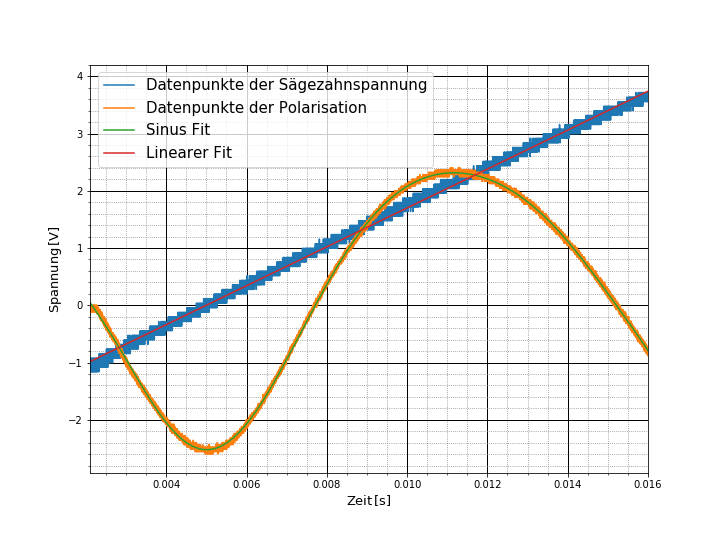
\includegraphics[scale=0.5]{Bild/V1_1}
	\centering
	\caption[Plot zu Versuchsteil 1]{\small Datenpunkte der ersten Messmethode mit Sägezahnspannung. In rot der Fit an die Steigung der Sägezahnkurve und in grün die Polynom Anpassung an die Datenpunkte der Photodiode.}
	\label{PoliBild}
\end{figure}
Von diesem wurde dann das Maximum und Minimum bestimmt. Mit den x-Werten dieser konnten nun die Spannungen der Sägezahnkurve bestimmt werden, indem sie in den Linearen Fit eingesetzt wurde:
\begin{equation}
	U_\text{Sägezahn}= mx_{\text{max/min}} + c
\end{equation}
Der Fehler auf die Spannung ergibt sich über Gaußsche Fehlerfortpflanzung durch Gleichung \ref{SägeSp}
\begin{equation}
	\sigma_{U_\text{Sägezahn}}=\sqrt{\left(mx_{\text{max/min}}\sigma_c\right)^2+\left((c + x_{\text{max/min}})\sigma_m\right)^2}
	\label{SägeSp}
\end{equation}
Nun können die beiden Werte der Spannung voneinander abgezogen werden und man erhält die Spannungsdifferenz $U_{\frac{\lambda}{2}}$. Der Fehler bekommt man durch:
\begin{equation}
	\sigma_{U_{\lambda/2}}=\sqrt{\left(U_\text{max}\sigma_{U_{\text{min}}}\right)^2+\left(U_{\text{min}}\sigma_{U_{\text{max}}}\right)^2}
	\label{Errdif}
\end{equation}
Da $15$ Messreihen erstellt wurde wird nun der Gewichtete Mittelwert dieser Werte genommen. Für dies wird Gleichung \ref{WMean} verwendet, der Fehler gibt sich wie in Gleichung \ref{Er_WMean}.
\begin{equation}
\bar{x}_g=\frac{\sum_ig_ix_i}{\sum_ig_i} \qquad \text{with} \qquad g_i=\frac{1}{\sigma_i^2}
\label{WMean}
\end{equation}
\begin{equation}
\sigma_{\bar{x}_g}=\frac{1}{\sqrt{\sum_i\nicefrac{1}{\sigma_i^2}}}
\label{Er_WMean}
\end{equation}
Als Wert ergibt sich für die Spannung dadurch $$U_{\frac{\lambda}{2}}=2.1278\pm0.0024\,\text{V}$$. Um nun die Elektrooptische Konstante $r_{41}$ zu bestimmen wird Gleichung \ref{r41} verwendet. Die Spannung muss davor jedoch noch um den Faktor $100$ vergrößert werden, da sie im Versuch um diesen Faktor gedämpft wurde. Die Werte für die Rechnung sind in der Versuchsanleitung \cite{anleitung} zu finden und wurden als fehlerfrei betrachtet. Damit ergab sich über die 1.Methode ein Wert von $$r_{41}=(26.489\pm0.030)\,\frac{\text{pm}}{V}$$\par
Die zweite Methode die Konstante zu bestimmen ist über Gleichspannung. Hierbei ist die Spannung die Differenz zwischen den beiden gemessenen Gleichspannungssignalen. Da sich diese sehr schlecht haben einstellen lassen wurden für positive so wie negative Spannung das Signal sechs mal gemessen. Aus diesen wir nun als erstes der Arithmetische Mittelwert bestimmt so wie dessen Fehler. Hierbei werden die Gleichungen \ref{Mean} und \ref{ErrMean} verwendet um den Fehler zu bestimmen.
\begin{equation}
\sigma_x = \frac{1}{n-1}\sum_{i=1}^{n}(x_i-\bar{x})^2
\label{Mean}
\end{equation}
\begin{equation}
	\sigma_{\bar{x}}=\frac{\sigma_x}{\sqrt{n}}
	\label{ErrMean}
\end{equation}
Mit dem Mittelwert der beiden Spannungen wird nun der die Differenz der beiden Bestimmt. Der Fehler berechnet sich hier wie bei der Gleichung \ref{Errdif}.
Damit ergibt sich als Wert für die Spannung $$U_{\frac{\lambda}{2}}=(255.60\pm0.30)\,\text{V}$$ 
Dies kann wie bei der ersten Methode in die Gleichung \ref{r41}
eingesetzt werden wodurch sich der Wert für die Elektrooptische Konstante von
$$r_{41}=(22.051\pm 0.026)\times\,\frac{\text{pm}}{\text{V}}$$
ergibt.

\subsection{Faraday Effekt}
Für die Auswertung des Faraday Effekts soll der Material abhängige Verdetkonstante bestimmt werden. Hierfür wird als erstes die Eingestellte Stromstärke gegen den gemessenen Drehwinkel aufgetragen. Die mit \verb|curve_fit| angepasste Gerade ist in Abbildung \ref{Dreh} zu finden. Die Geradengleichung lautet:
$$\alpha=(2.642\pm0.021)\,\frac{\circ}{\text{A}}\cdot I + (0.70\pm0.06)^\circ$$
\begin{figure}[ht]
	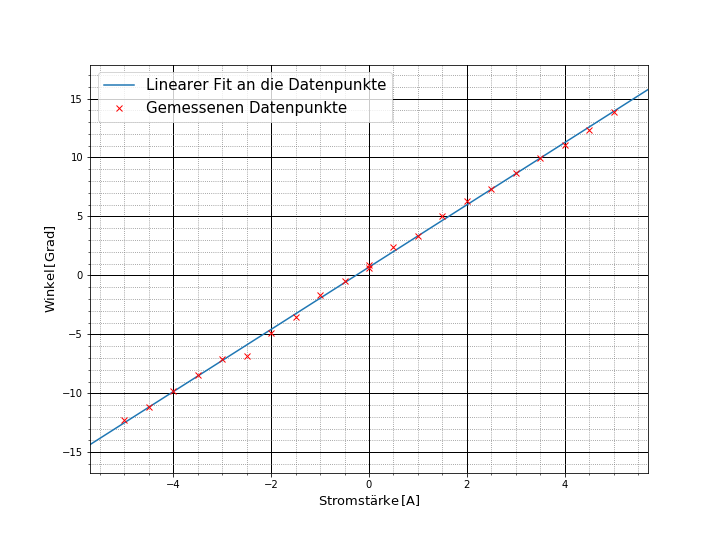
\includegraphics[scale=0.5]{Bild/V2Lin}
	\centering
	\caption[Datenpunkte und Fit der Faraday Messung]{\small In rot die gemessenen Datenpunkte und in blau der lineare Fit an diese. Es wurden keine Fehler mit eingezeichnet da diese zu klein waren um sie sinnvoll darzustellen.}
	\label{Dreh}
\end{figure}
Nun wird einmal für eine reale und eine ideale Spule die Verdetkonstante bestimmt.\par
Für eine reale Spule kann man Gleichung \ref{real} nehmen. Hierbei ist $\frac{\alpha}{I}$ gerade die Steigung der Geraden und der Faktor $2556$ ein Wert der im Staatsexamen\cite{staatsexamen} mit der Gleichung \ref{realFormel} für eine reale Spule berechnet wurde.
\begin{equation}
	V_{real}=\frac{\alpha}{\text{A}\cdot 2556}
	\label{real}
\end{equation}
Damit ergibt sich ein Wert für die Konstante von $$V_{real}=(0.001034 \pm 0.000008)\,\frac{\circ}{\text{A}}$$
Für eine ideale Spule wird die Gleichung \ref{idealH} verwendet.
\begin{equation}
	V_{ideal}=\frac{\alpha}{\text{A}}\frac{L}{Nl}\approx \frac{\alpha}{\text{A}\cdot 3086}
	\label{idealH}
\end{equation}
Hierbei ist $L$ die Länge der Spule $l$ die Länge des Materials in der Spule und $N$ die Anzahl der Windungen. Werte sind in der Versuchsanleitung zu finden\cite{anleitung}. Hier ergibt sich für die Verdetkonstante ein Wert von:
$$V_{ideal}=(0.000856 \pm 0.000007)\,\frac{\circ}{\text{A}}$$
Um diese mit der Angabe des Herstellers von $V_{HS}=0.05\,\frac{\text{min}}{\text{Oe cm}}$ zu vergleichen müssen die Werte umgerechnet werden dabei gilt:
$$1\,\text{A}=\frac{100}{79.59}\,\text{Oe cm}  \qquad \qquad 1\,\text{Grad}=60\,\text{min}$$
Damit ergeben sich die Werte von:
$$V_{real}=(0.0494 \pm 0.0004)\,\frac{\text{min}}{\text{Oe cm}}$$
$$V_{ideal}=(0.04088 \pm 0.00032)\,\frac{\text{min}}{\text{Oe cm}}$$